
\section{\trigsub{Trigonometric Substitution}}

Though in theory you could use any trigonometric function, the three commonly used \trigfunctions{\integ{trigonometric substitutions}} are sine, tangent, and secant.  The substitutions are motivated by the Pythagorean Identities from trigonometry.

\begin{exercise}{Recalling the Pythagorean Identities \Coffeecup} 
\begin{itemize}
\item Start with the \trigidentities{Pythagorean Identity} for sine and cosine: $$\cos^2\left(\theta\right)+\sin^2\left(\theta\right)=1 $$
\item Subtract $\sin^2\left(\theta\right) $ from both sides.  Write the resulting equation below.
\solushun{$$\cos^2(\theta)=1-\sin^2(\theta)$$}{.2in}
\item Again, start with the Pythagorean Identity for sine and cosine.  What would we have to divide both sides by in order to get the corresponding identity for tangent and secant (written below)?
$$1+\tan^2\left(\theta\right)=\sec^2\left(\theta\right) $$
\solushun{Divide everything by $\cos^2(\theta)$
$$\frac{\cos^2\left(\theta\right)}{\cos^2\left(\theta\right)}+\frac{\sin^2\left(\theta\right)}{\cos^2\left(\theta\right)}=\frac{1}{\cos^2\left(\theta\right)}$$
$$1+\tan^2\left(\theta\right)=\sec^2\left(\theta\right)$$}{.2in}
\item How would you then obtain the identity below?
$$\sec^2\left(\theta\right)-1=\tan^2\left(\theta\right) $$
\solushun{Subtract $1$ from both sides.\\}{.2in}
\end{itemize}
\end{exercise}

You can take any of the identities above and multiply both sides by $a^2$ (where $a$ represents an arbitrary positive real constant) to produce a more general identity.  This is what results in the commonly used \antider{trigonometric substitutions} for integrals, summarized in the table below.

\FormulaBox{Trigonometric Substitutions}{
\begin{tabular}{c|c|c} \hline 
 If you see... &   ...make the substitution... & ...because...  \\ \hline 
 $a^2-x^2$ &  $  x=a \sin\left(\theta\right) $ & $a^2-a^2\sin^2\left(\theta\right)=a^2\cos^2\left(\theta\right) $ \\
 $a^2+x^2$ &  $  x=a \tan\left(\theta\right) $ & $a^2+a^2\tan^2\left(\theta\right)=a^2\sec^2\left(\theta\right) $ \\
$x^2-a^2$ &  $  x=a \sec\left(\theta\right) $ & $a^2\sec^2\left(\theta\right)-a^2=a^2\tan^2\left(\theta\right) $ \\
\end{tabular}}

\begin{exercise}{Why Only Three Cases? \Coffeecup} In the table above, we have cases for how to clean up expressions of the form $a^2-x^2$, $a^2+x^2$, and $x^2-a^2$.  Why is there not a fourth case for $x^2+a^2$?
\solushun{The case $x^2+a^2$ is equivalent to the case $a^2+x^2$, so we can rearrange the expression and use the substitution $x=a\tan(\theta)$\\}{.2in}
\end{exercise}%
%
\subsection{\sine{Sine Substitution}} When we see an expression of the form $a^2-x^2$ in the integrand, we think of the identity $1-\sin^2(\theta)=\cos^2(\theta)$.  This motivates the following substitution:

\FormulaBox{Sine Substitution}{\begin{tabular}{c}
		$x=a\cdot \sin(\theta)$
	\end{tabular}
}

The next example will require use of the \trigidentities{Double-Angle Identities} for sine and cosine.  We recall these before we dive in!

\begin{exercise}{Recalling the Double-Angle Formulas \Coffeecup}
\begin{itemize}
\item The double-angle formula for sine is $\sin(2\theta)=$
\solushun{$\sin(2\theta)=2\sin(\theta)\cos(\theta)$\\}{0in}
\item The double-angle formula for cosine is $\cos(2\theta)=$
\solushun{$\cos(2\theta)=\cos^2(\theta)-\cos^2(\theta)$\\}{0in}
\item What do you get if you apply the sine double-angle identity to $\sin(4\theta)$?  Specifically, think of $\sin(4\theta)$ as $\sin\left(2\cdot 2\theta \right)$. 
\solushun{$\sin(4\theta)=2\sin(2\theta)\cos(2\theta)$\\}{.2in}\vspace*{.2in}
\end{itemize}
\end{exercise}

We now put our sine substitution to use to evaluate an antiderivative!
\begin{example}{Using a Sine Substitution}
 Suppose we wish to evaluate $$\int \left( 4-x^2 \right)^{3/2} \dif x$$
  
We use the substitution suggested above, specifically $$x=2\cdot \sin(\theta).$$  We then differentiate both sides to find the conversion between the differentials and then multiply both sides by $\dif \theta$: $$ \frac{\dif x}{\dif \theta}=2 \cdot \cos(\theta) $$

We now use the above equations to substitute for $x$ and $\dif x$ in the integral:

\begin{align*} \int \left( 4-x^2 \right)^{3/2} \mathtt{d}x &=\int \left( 4-(2\cdot \sin(\theta))^2 \right)^{3/2} 2\cdot \cos(\theta)\mathtt{d}\theta \\
&=2 \int \left(4-4\cdot \sin^2(\theta)\right)^{3/2}\cos(\theta) \mathtt{d}\theta \\
&=2 \int \left(4\left(1-\sin^2(\theta)\right)\right)^{3/2}\cos(\theta) \mathtt{d}\theta \\
&=2 \int \left(4\left(\cos^2(\theta)\right)\right)^{3/2}\cos(\theta) \mathtt{d}\theta \\
&=2 \int \left(4\right)^{3/2}\left(\cos^2(\theta)\right)^{3/2}\cos(\theta) \mathtt{d}\theta
\\
&=16 \int \cos^3(\theta)\cdot \cos(\theta) \mathtt{d}\theta
\\
&=16 \int \cos^4(\theta) \mathtt{d}\theta
\end{align*}

Recall the previous section where we learned how to antidifferentiate even powers of sine and cosine!  Accordingly, we use the half-angle identities.

\begin{align*} \int \left( 4-x^2 \right)^{3/2} \mathtt{d}x &=16 \int \left(\cos^2(\theta)\right)^2 \mathtt{d}\theta \\
&=16 \int \left(\frac{1+\cos(2\theta)}{2}\right)^2 \mathtt{d}\theta \\
&=16 \int \frac{1+2\cdot \cos(2\theta)+\cos^2(2\theta)}{4} \mathtt{d}\theta \\
&=4 \int 1+2\cdot \cos(2\theta)+\cos^2(2\theta) \mathtt{d}\theta \\
&=4 \int 1+2\cdot \cos(2\theta)+\frac{1+\cos(4\theta)}{2} \mathtt{d}\theta \\
&=4 \int \frac{3}{2}+2\cdot \cos(2\theta)+\frac{1}{2}\cos(4\theta) \mathtt{d}\theta \\
&=4 \left( \frac{3}{2}\theta +\sin(2\theta) +\frac{1}{8}\sin(4\theta) \right)+C \\
&=6\theta +4\cdot \sin(2\theta) +\frac{1}{2}\sin(4\theta)+C
\end{align*}

We have successfully taken the antiderivative!  However, it still remains to unwind the \doubleangle{trigonometric substitution} back in terms of $x$ rather than $\theta$.  Our original substitution argument is $\theta$, whereas currently we have $2\theta $ and $4\theta $ as arguments.  In order to resolve this, we use the sine and cosine double angle formulas and the Pythagorean identity.  Proceeding:
\begin{align*} \int \left( 4-x^2 \right)^{3/2} \mathtt{d}x &=6\theta +4\cdot \sin(2\theta) +\frac{1}{2}\sin(4\theta)+C \\
&=6\theta +4\cdot 2\cdot \sin(\theta)\cos(\theta) + \sin(2\theta)\cos(2\theta)+C \\
&=6\theta +4\cdot 2\cdot \sin(\theta)\cos(\theta) +2\cdot \sin(\theta)\cos(\theta)\left(\cos^2(\theta)-\sin^2(\theta)\right)+C \\
&=6\theta +8\cdot \sin(\theta)\sqrt{1-\sin^2(\theta)} +2\cdot \sin(\theta)\sqrt{1-\sin^2(\theta)}\left(1-2\sin^2(\theta)\right)+C \\
&=6\cdot \arcsin\left(\frac{x}{2}\right)+8\frac{x}{2}\sqrt{1-\frac{x^2}{4}}+2\frac{x}{2}\sqrt{1-\frac{x^2}{4}}\left(1-2\frac{x^2}{4}\right)+C \\
&=6\cdot \arcsin\left(\frac{x}{2}\right)+4x\sqrt{1-\frac{x^2}{4}}+\sqrt{1-\frac{x^2}{4}}\left(x-\frac{x^3}{2}\right)+C
\end{align*}

\end{example}
 \begin{exercise}{Checking Our Work \Coffeecup \Coffeecup \Coffeecup }
Verify the result of the previous example by differentiating! 
\solushun{First apply all the product and chain rules to reach the expression $$\frac{3}{\sqrt{1-\frac{x^2}{4}}}+4\sqrt{1-\frac{x^2}{4}}+\frac{-x^2}{\sqrt{1-\frac{x^2}{4}}}+\sqrt{1-\frac{x^2}{4}}\left(1-\frac{3}{2}x^2\right)+\frac{-x}{4\sqrt{1-\frac{x^2}{4}}}\left(x-\frac{x^3}{2}\right) $$  Put all terms over the common denominator $\sqrt{4-x^2}$ and combine like terms in the numerator.
\begin{align*}
&=\frac{3\cdot2}{\sqrt{4-x^2}}+\frac{2\cdot 4\left(1-\frac{x^2}{4}\right)-2x^2}{\sqrt{4-x^2}}+\frac{4(1-\frac{x^2}{4})\left(1-\frac{3}{2}x^2\right)-x\left(x-\frac{x^3}{2}\right)}{4\sqrt{1-\frac{x^2}{4}}}\\
&=\frac{6}{\sqrt{4-x^2}}+\frac{8-2x^2-2x^2}{\sqrt{4-x^2}}+\frac{4-6x^2-x^2+\frac{3}2{x^4}-x^2+\frac{x^4}{2}}{4\sqrt{1-\frac{x^2}{4}}}\\
&=\frac{6}{\sqrt{4-x^2}}+\frac{8-4x^2}{\sqrt{4-x^2}}+\frac{2-4x^2+{x^4}}{\sqrt{4-x^2}}\\
&=\frac{16-8x^2+x^4}{\sqrt{4-x^2}}\\
&=\frac{\left(4-x^2\right)^2}{\sqrt{4-x^2}}\\
&=\left(4-x^2\right)^\frac{3}{2}
\end{align*}}{3in}
\AnswerKeyEntry{First apply all the product and chain rules to reach the expression $$\frac{3}{\sqrt{1-\frac{x^2}{4}}}+4\sqrt{1-\frac{x^2}{4}}+\frac{-x^2}{\sqrt{1-\frac{x^2}{4}}}+\sqrt{1-\frac{x^2}{4}}\left(1-\frac{3}{2}x^2\right)+\frac{-x}{4\sqrt{1-\frac{x^2}{4}}}\left(x-\frac{x^3}{2}\right) $$  Put all terms over the common denominator $\sqrt{4-x^2}$ and combine like terms in the numerator.  Notice the numerator becomes $\left(4-x^2\right)^2$ and then reduce for the win!}
\end{exercise}
\subsubsection{An Alternate Approach}
In the above example, we made it back from $\theta$ to $x$ by just bashing it to bits with trig identities.  Sometimes a cleaner approach can be to use a little geometry.  Since we had the substitution $x=2\sin(\theta)$, we can divide both sides by 2 to obtain the following:  $$\sin(\theta)=\frac{x}{2}$$ 

Since sine is the ratio of the opposite side to the hypotenuse in a right triangle, we can label the opposite side as $x$ and the hypotenuse as 2. 
\begin{center}
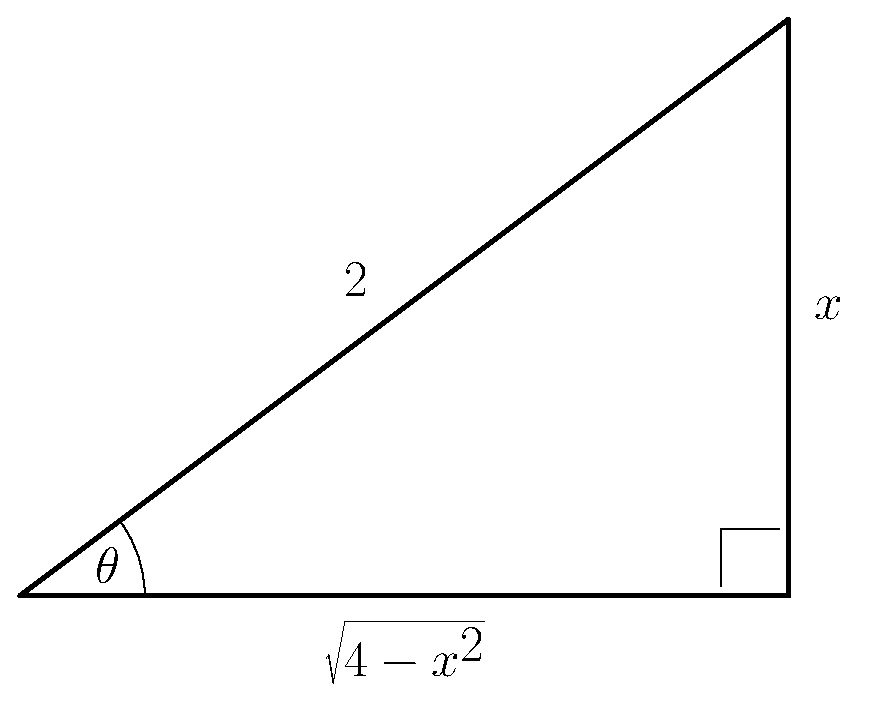
\includegraphics[scale=0.4]{ChapterAntidiff/Figures/sinsubtri}
\end{center}
This makes it easier to know what to substitute for other trig functions of $\theta$.  For example, cosine is the ratio of the adjacent side length to the hypotenuse, so we have:
$$\cos(\theta)=\frac{\sqrt{4-x^2}}{2} $$


\begin{exercise}{
Try One on your own! \Coffeecup \Coffeecup \Coffeecup}
 Evaluate the following antiderivative:

$$\int x^3\left( 16-x^2 \right)^{5/2} \dif x$$  ({\bf Hint:} Recall our methods for integrating powers of sines and cosines!)
\solushun{We have an expression of the form $a^2-x^2$, so we can use a sine substitution and let $x=4\sin(\theta), \dif x=4\cos(\theta)\dif\theta$.
\begin{align*}
\int x^3\left(16-x^2\right)^\frac{5}{2}\dif x&=\int \left(4\sin(\theta)\right)^3\left(16-16\sin^2(\theta)\right)^\frac{5}{2}4\cos(\theta)\dif\theta\\
&=\int 4^3\sin^3(\theta)\left(16\left(1-\sin^2(\theta)\right)\right)^\frac{5}{2}4\cos(\theta)\dif\theta\\
&=\int 4^3\sin^3(\theta)\cdot4^5\left(\cos^2(\theta)\right)^\frac{5}{2}\cdot4\cos(\theta)\dif\theta\\
&=4^9\int \sin^3(\theta)\cdot\cos^5(\theta)\cdot\cos(\theta)\dif\theta\\
&=4^9\int \sin^3(\theta)\cos^6(\theta)\dif\theta\\
\end{align*}
Now we can use our tools for integrating powers of sine and cosine, with $u=\cos(\theta)$ and $\dif u =-\sin(\theta)$.
\begin{align*}
4^9\int \sin^3(\theta)\cos^6(\theta)\dif\theta&=4^9\int \left(\sin^2(\theta)\right)\left(\sin(\theta)\right)\cos^6(\theta)\dif\theta\\
&=4^9\int \left(1-\cos^2(\theta)\right)\left(\sin(\theta)\right)\cos^6(\theta)\dif\theta\\
&=-4^9\int \left(1-u^2\right)u^6\dif u\\
&=-4^9\int u^6-u^8\dif u\\
&=-4^9\left(\frac{1}{7}u^7-\frac{1}{8}u^8\right)+C\\
&=-4^9\left(\frac{1}{7}\cos^7(\theta)-\frac{1}{9}\cos^9(\theta)\right)+C\\
\end{align*}
\begin{wrapfigure}{r}{0.25\textwidth}
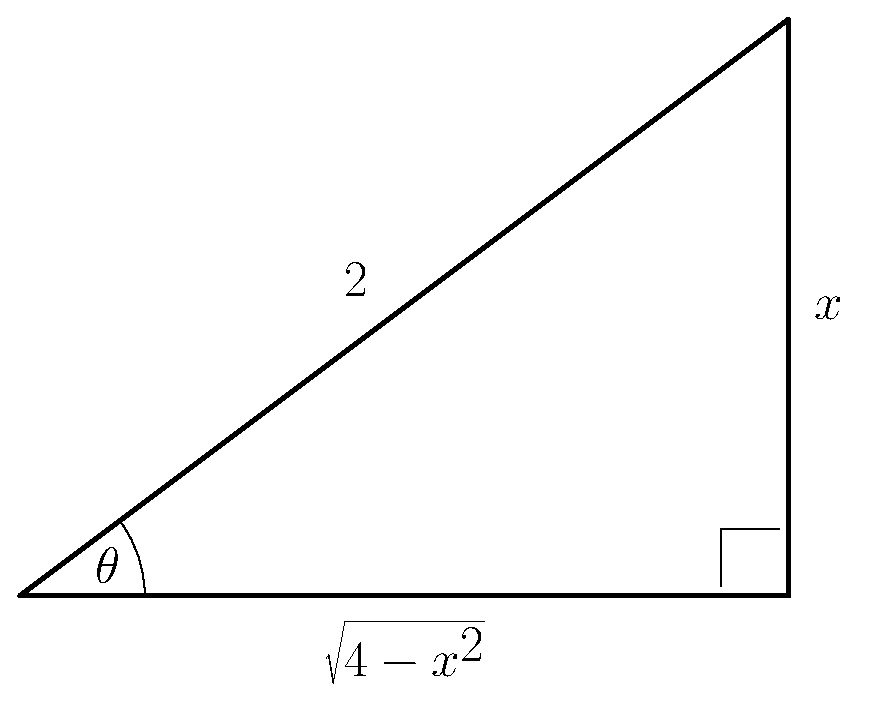
\includegraphics[scale=0.3]{ChapterAntidiff/Figures/sinsubtri}
\end{wrapfigure}
To unwind in terms of $x$, we can use the definition of sine and cosine as side ratios of a triange. If $x=4\sin(\theta)$, we can draw the triangle:\\
From this, you can see that $\cos(\theta)=\frac{\sqrt{4^2-x^2}}{4}$. We can substitute that in for the $\cos(\theta)$'s in the answer:
\begin{align*}
-4^9\left(\frac{1}{7}\cos^7(\theta)-\frac{1}{9}\cos^9(\theta)\right)+C&=-4^9\left(\frac{1}{7}\left(\frac{\sqrt{4^2-x^2}}{4}\right)^7-\frac{1}{9}\left(\frac{\sqrt{4^2-x^2}}{4}\right)^9\right)+C\\
&=-4^9\left(\frac{1}{7}\left(\frac{4\sqrt{1-\frac{x^2}{16}}}{4}\right)^7-\frac{1}{9}\left(\frac{4\sqrt{1-\frac{x^2}{16}}}{4}\right)^9\right)+C\\
&=-4^9\left(\frac{1}{7}\left(\sqrt{1-\frac{x^2}{16}}\right)^7-\frac{1}{9}\left(\sqrt{1-\frac{x^2}{16}}\right)^9\right)+C\\
&=2^{18}\left(\frac{\left(1-\frac{x^2}{16}\right)^{9/2}}{9}-\frac{\left(1-\frac{x^2}{16}\right)^{7/2}}{7}\right)+C\\
\end{align*}
And that's it.
}{3in}
\AnswerKeyEntry{The antiderivative is $2^{18}\left(\frac{\left(1-x^2/16\right)^{9/2}}{9}-\frac{\left(1-x^2/16\right)^{7/2}}{7}\right)+C$}
\end{exercise} 

\subsection{\secant{Secant Substitution}}\label{secantsub} When we see an expression of the form $x^2-a^2$ in the integrand, we think of the identity $\sec^2(\theta)-1=\tan^2(\theta)$, so we use the following substitution:

\FormulaBox{Secant Substitution}{\begin{tabular}{c}
		$x=a\cdot \sec(\theta)$
	\end{tabular}}
    
\begin{example}{A Secant Substitution}\label{secsub}
Suppose we wish to evaluate the following integral: $$\int \frac{1}{x^4-9x^2}\dif x $$  Since $x^4-9x^2=x^2\left(x^2-9\right)$, we use the following substitution: 
\begin{align*}
x&=3\sec\left(\theta\right) \\
\dif x &= 3 \sec\left(\theta\right)\tan\left(\theta\right)\dif \theta 
\end{align*}

We now apply these substitutions to rewrite the integral in terms of $\theta$.

\begin{align*}
\int \frac{1}{x^4-9x^2}\dif x &=\int \frac{1}{x^2\left(x^2-9\right)}\dif x  \\
&=\int \frac{3 \sec\left(\theta\right)\tan\left(\theta\right)}{9\sec^2\left(\theta\right)\left(9\sec^2\left(\theta\right)-9\right)}\dif \theta \\
&=\int \frac{3 \sec\left(\theta\right)\tan\left(\theta\right)}{81\sec^2\left(\theta\right)\tan^2\left(\theta\right)}\dif \theta \\
&=\frac{1}{27}\int \frac{1}{\sec\left(\theta\right)\tan\left(\theta\right)}\dif \theta \\
&=\frac{1}{27}\int\frac{\cos^2\left(\theta\right)}{\sin\left(\theta\right)} \dif \theta \\
&=\frac{1}{27}\int\frac{1-\sin^2\left(\theta\right)}{\sin\left(\theta\right)} \dif \theta \\
&=\frac{1}{27}\int\frac{1}{\sin\left(\theta\right)} \dif \theta-\frac{1}{27}\int \frac{\sin^2\left(\theta\right)}{\sin\left(\theta\right)}\dif \theta \\
&=\frac{1}{27}\int \csc\left(\theta\right) \dif \theta -\frac{1}{27}\int \sin\left(\theta\right) \dif \theta \\
&=-\frac{1}{27}\ln\left|\csc\left(\theta\right)+\cot\left(\theta\right)\right|+\frac{1}{27}\cos\left(\theta\right)+C
\end{align*}
Here we have successfully taken the antiderivative, and now need to just get back to $x$ from $\theta$.  We draw a triangle and label the sides according to our substitution.  In particular, $$\sec\left(\theta\right)=\frac{x}{3}=\frac{\text{hypotenuse}}{\text{adjacent}}$$ so we can let the hypotenuse be $x$ and the adjacent side be 3.
\begin{center}
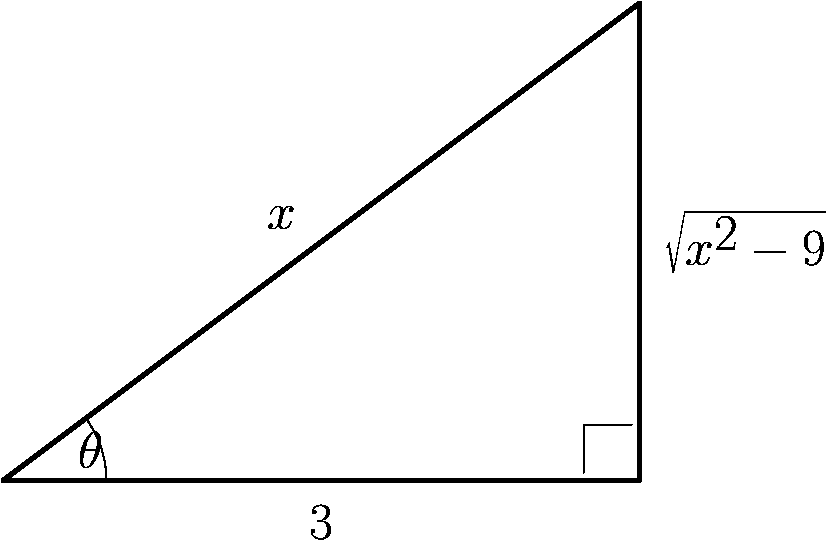
\includegraphics[scale=0.4]{ChapterAntidiff/Figures/sectri_crop}
\end{center}
This enables us to compute the other trig functions using this triangle.  
\end{example}

\begin{exercise}{Getting from $\theta$ back to $x$ \Coffeecup }
Complete the above example by using the triangle to find the values of the other trig functions. \vspace{-.3in}
\begin{center}
\begin{align*}
\cos(\theta)&= \hspace{2in}\\
\cot(\theta)&= \hspace{2in}\\
\csc(\theta)&= \hspace{2in}
\end{align*}
\end{center}

Then plug these expressions back into our antiderivative to get a final answer in terms of $x$ rather than $\theta$.  Make these substitutions and then simplify to verify the final answer shown below.  Show your work below.  \begin{align*}
\int \frac{1}{x^4-9x^2}\dif x &= -\frac{1}{27}\ln\left|\csc\left(\theta\right)+\cot\left(\theta\right)\right|+\frac{1}{27}\cos\left(\theta\right)+C \\
&= \\
&= \\
&= \frac{1}{9x}-\frac{1}{27}\ln\left| \frac{x+3}{\sqrt{x^2-9}}\right|+C
\end{align*}

\end{exercise}

\begin{exercise}{Yes You Can!  Take the Cant Out of Secant! \Coffeecup \Coffeecup \Coffeecup} Evaluate the following antiderivative:
$$\int \sqrt{x^2-4}\dif x.$$
\solushun{We have an expression of the form $x^2-a^2$, so we can use a secant substitution and let $x=2\sec(\theta), \dif x=2\sec(\theta)\tan(\theta)\dif\theta$.
\begin{align*}
\int \sqrt{x^2-4}\dif x&=\int \sqrt{4\sec^2(\theta)-4}\cdot2\sec(\theta)\tan(\theta)\dif \theta\\
&=\int \sqrt{4\sec^2(\theta)-4}\cdot2\sec(\theta)\tan(\theta)\dif \theta\\
&=\int 2\sqrt{\sec^2(\theta)-1}\cdot2\sec(\theta)\tan(\theta)\dif \theta\\
&=4\int \sqrt{\tan^2(\theta)}\cdot\sec(\theta)\tan(\theta)\dif \theta\\
&=4\int \sec(\theta)\tan^2(\theta)\dif \theta\\
\end{align*}
Using the Pythagorean Identity, we can split the integral:
\begin{align*}
4\int \sec(\theta)\tan^2(\theta)\dif \theta&=4\int \sec(\theta)\left(\sec^2(\theta)-1\right)\dif \theta\\
&=4\int \sec^3(\theta)-\sec(\theta)\dif \theta\\
&=4\left[\int \sec^3(\theta)\dif \theta-\int \sec(\theta)\dif \theta\right]
\end{align*}
From previous exercises, we can evaluate these as:
$$
4\left[\int \sec^3(\theta)\dif \theta-\int \sec(\theta)\dif \theta\right]=4\left[\frac{\sec(\theta)\tan(\theta)+\ln\left|\sec(\theta)+\tan(\theta)\right|}{2}-\ln\left|\sec(\theta)+\tan(\theta)\right|\right]
$$
To unwind, note that $x=2\sec(\theta)$ so that $\sec(\theta)=\frac{x}{2}$, which gives us enough information to draw a right triangle (try it) and find the side ratios, giving us $\tan(\theta)=\frac{\sqrt{x^2-4}}{2}$.
\begin{align*}
4\left[\frac{\sec(\theta)\tan(\theta)+\ln\left|\sec(\theta)+\tan(\theta)\right|}{2}-\ln\left|\sec(\theta)+\tan(\theta)\right|\right]+C\\
=4\left[\frac{\frac{x}{2}\cdot\frac{\sqrt{x^2-4}}{2}+\ln\left|\frac{x}{2}+\frac{\sqrt{x^2-4}}{2}\right|}{2}-\ln\left|\frac{x}{2}+\frac{\sqrt{x^2-4}}{2}\right|\right]+C\\
=4\left[\frac{\frac{x\sqrt{x^2-4}}{4}+\ln\left|\frac{x+\sqrt{x^2-4}}{2}\right|}{2}-\ln\left|\frac{x+\sqrt{x^2-4}}{2}\right|\right]+C\\
=\frac{x\sqrt{x^2-4}}{2}+2\ln\left|\frac{x+\sqrt{x^2-4}}{2}\right|-4\ln\left|\frac{x+\sqrt{x^2-4}}{2}\right|+C\\
=\frac{x\sqrt{x^2-4}}{2}-2\ln\left|\frac{x+\sqrt{x^2-4}}{2}\right|+C
\end{align*}
We can clean this up a bit by absorbing part of the logarithm into the constant:
\begin{align*}
\frac{x\sqrt{x^2-4}}{2}-2\ln\left|\frac{x+\sqrt{x^2-4}}{2}\right|+C&=\frac{x\sqrt{x^2-4}}{2}-\left(2\ln\left|x+\sqrt{x^2-4}\right|-2\ln|2|\right)+C\\
&=\frac{x\sqrt{x^2-4}}{2}-2\ln\left|x+\sqrt{x^2-4}\right|+C
\end{align*}}{4in}
\AnswerKeyEntry{Exercise \ref{reappear}.\ref{seccubed} will be helpful!  The antiderivative is $\frac{x\sqrt{x^2-4}}{2}-2\ln|x+\sqrt{x^2-4}|+C$.}
\end{exercise}

\subsection{\tangent{Tangent Substitution}} When we see an expression of the form $a^2+x^2$ or $x^2+a^2$ (which are the same) in the integrand, we think of the identity $\tan^2(\theta)+1=\sec^2(\theta)$, so we use the following substitution:

\FormulaBox{Tangent Substitution}{\begin{tabular}{c}
		$x=a\cdot \tan(\theta)$
	\end{tabular}
}

\begin{exercise}{Revisiting an Old Friend \Coffeecup \Coffeecup}
\begin{itemize}
\item Recall the derivative of arctangent:
$$\frac{\dif}{\dif x}\left(\arctan(x)\right)=\hspace{3in} $$
\solushun{$$\frac{1}{1+x^2}$$}{0in}

\item We should be able to reverse the above by taking the antiderivative of the right-hand side.  Perform this antiderivative using the substitution $x=\tan(\theta)$:

$$\int \frac{1}{1+x^2}\dif x = \hspace{3.2in} $$
\solushun{Let $x=\tan(\theta), \dif x=\sec^2(\theta)$.
\begin{align*}
\int \frac{1}{1+x^2}\dif x&=\int \frac{1}{1+tan^2(\theta)}\sec^2(\theta)\dif\theta\\
&=\int \frac{\sec^2(\theta)}{\sec^2(\theta)}\dif\theta\\
&=\int 1\dif\theta\\
&=\theta+C\\
&=\arctan(x)+C
\end{align*}}{2in}

\end{itemize}
\end{exercise}

\subsection{Preprocessing with Algebra or $u$-sub}  Often we need to do a little algebra and/or $u$-sub to get the integrand into a form where we can then perform trig sub.


\begin{exercise}{A Bit of Algebra to Help Us \Coffeecup \Coffeecup \Coffeecup }

\begin{itemize}
\item Explain why the two following expressions are equal: $$(4x^2+1)^2=16\left(x^2+\left(\frac{1}{2}\right)^2\right)^2$$
\solushun{\begin{align*}
(4x^2+1)^2&=\left(4\left(x^2+\frac{1}{4}\right)\right)^2\\
&=\left(4\right)^2\left(x^2+\left(\frac{1}{2}\right)^2\right)^2\\
&=16\left(x^2+\left(\frac{1}{2}\right)^2\right)^2
\end{align*}}{1in}

\item Use the equality above along with a tangent substitution to evaluate the following antiderivative:

$$\int \frac{1}{(4x^2+1)^2} \dif x$$
\solushun{\begin{align*}
\int \frac{1}{(4x^2+1)^2} \dif x&=\int \frac{1}{16\left(x^2+\left(\frac{1}{2}\right)^2\right)^2} \dif x\\
&\text{Let $x=\frac{1}{2}\tan(\theta), \dif x=\frac{1}{2}\sec^2(\theta)$}.\\
&=\int \frac{1}{16\left(\frac{1}{4}\tan^2(\theta)+\left(\frac{1}{2}\right)^2\right)^2}\cdot\frac{1}{2}\sec^2(\theta)\dif\theta\\
&=\frac{1}{32}\int \frac{\sec^2(\theta)}{\left(\frac{1}{4}\tan^2(\theta)+\left(\frac{1}{2}\right)^2\right)^2}\dif\theta\\
&=\frac{1}{32}\int \frac{\sec^2(\theta)}{\left(\frac{1}{4}\sec^2(\theta)\right)^2}\dif\theta\\
&=\frac{1}{32}\int \frac{\sec^2(\theta)}{\frac{1}{16}\sec^4(\theta)}\dif\theta\\
&=\frac{1}{2}\int \frac{1}{\sec^2(\theta)}\dif\theta\\
&=\frac{1}{2}\int \cos^2(\theta)\dif\theta\\
&=\frac{1}{2}\int \frac{1+\cos(2\theta)}{2}\dif\theta\\
&=\frac{1}{2}\int \frac{1}{2}+\frac{1}{2}\cos(2\theta)\dif\theta\\
&=\frac{1}{2}\left( \frac{1}{2}\theta+\frac{1}{4}\sin(2\theta)+C\right)\\
&= \frac{1}{4}\theta+\frac{1}{8}\sin(2\theta)+C\\
&= \frac{1}{4}\theta+\frac{1}{4}\sin(\theta)\cos(\theta)+C\\
&\text{Since, $\tan(\theta)=2x$, we construct a triangle to obtain $\cos(\theta)$ and $\sin(\theta)$.}\\
&\sin(\theta))=\frac{2x}{\sqrt{4x^2-1}}, \cos(\theta))=\frac{1}{\sqrt{4x^2-1}}\\
&=\frac{1}{4}\arctan(2x)+\frac{1}{4}\frac{2x}{\sqrt{4x^2-1}}\cdot\frac{1}{\sqrt{4x^2-1}}+C\\
&=\frac{1}{4}\arctan(2x)+\frac{x}{8x^2-2}+C\\
\end{align*}}{4in}
\end{itemize}
\end{exercise}

A trick from algebra that is often used \cts{with trigonometric substitution} is completing the square.  You might need to complete the square to get it into a form where a trig sub will work.  

\begin{example}{Completing the Square}
Suppose we wish to find an antiderivative for the function $\left(x^2+x-1\right)^{-2}$.  We begin by completing the square on the quadratic polynomial:

\begin{align*}
x^2+x-1&=x^2+x+\frac{1}{4}-\frac{1}{4}-1 \\
       &=\left(x+\frac{1}{2}\right)^2-\frac{5}{4} \\ 
\end{align*}

We now use the substitution that this quadratic motivates.  Namely, we pick $a=\frac{\sqrt{5}}{2}$ since we want its square to be five-fourths.  Where $x$ used to go in the problems above, we now have an $x+\frac{1}{2}$.  Thus our substitution is $ x+\frac{1}{2}=\frac{\sqrt{5}}{2}\sec(\theta)$, or more explicitly:

$$  x=\frac{\sqrt{5}}{2}\sec(\theta)-\frac{1}{2} $$

Taking the derivative of both sides with respect to $\theta$ shows that 

$$  \mathtt{d}x=\frac{\sqrt{5}}{2}\sec(\theta)\tan(\theta) \mathtt{d}\theta $$

\end{example}

\begin{exercise}{Completing the Example \Coffeecup \Coffeecup \Coffeecup}

Use the substitutions suggested in the example above to find the antiderivative.

$$\int \frac{1}{(x^2+x-1)^2} \mathtt{d}x = \hspace{4in} $$

\AnswerKeyEntry{The antiderivative is $-\frac{1}{5}\frac{2x+1}{x^2+x-1}+\frac{4\sqrt{5}}{25}\ln\left(\frac{2x+1+\sqrt{5}}{2\sqrt{x^2+x-1}}\right)+C$.  Note that one can expand using properties of logarithms and then rename $C$ as $C-\frac{4\sqrt{5}}{25}\ln(2)$ since it is anyhow just an arbitrary constant.  Thus, we can slightly clean up the answer to become $-\frac{1}{5}\frac{2x+1}{x^2+x-1}+\frac{4\sqrt{5}}{25}\ln\left(2x+1+\sqrt{5}\right)-\frac{2\sqrt{5}}{25}\ln\left(x^2+x-1\right)+C.$}

\solushun{With $x+\frac{1}{2}=\frac{\sqrt{5}}{2}\sec(\theta)$, and $\dif x=\frac{\sqrt{5}}{2}\sec(\theta)\tan(\theta) \dif\theta$, we have:
\begin{align*}
\int \frac{1}{(x^2+x-1)^2} \dif x &= \int \frac{1}{(x+\frac{1}{2})^2-\frac{5}{4}} \dif x = \int \frac{\frac{\sqrt{5}}{2}\sec(\theta)\tan(\theta)}{\left(\frac{\sqrt{5}}{2}\sec(\theta)\right)^2-\frac{5}{4}} \dif\theta \\
&=\frac{\sqrt{5}}{2}\int \frac{\sec(\theta)\tan(\theta)}{\frac{5}{4}\sec^2(\theta)-\frac{5}{4}} \dif\theta\\
&=\frac{2\sqrt{5}}{5}\int \frac{\sec(\theta)\tan(\theta)}{\tan^2(\theta)} \dif\theta\\
&=\frac{2\sqrt{5}}{5}\int \frac{\sec(\theta)}{\tan(\theta)} \dif\theta\\
&=\frac{2\sqrt{5}}{5}\int\csc(\theta)\dif\theta\\
&=-\frac{2}{\sqrt{5}}\ln|\csc(\theta)+\cot(\theta)|+C\\
\end{align*}
Using the initial substitution $\sec(\theta)=\frac{2}{\sqrt{5}}\left(x+\frac{1}{2}\right)$, we can draw a triangle and derive the other sides to get $\csc\theta=\frac{2x+1}{2\sqrt{x^2+x-1}}$ and $\cot\theta=\frac{\sqrt{5}}{2\sqrt{x^2+x-1}}$
\begin{align*}
-\frac{2}{\sqrt{5}}\ln\left|\csc(\theta)+\cot(\theta)\right|+C&=-\frac{2}{\sqrt{5}}\ln\left|\frac{2x+1}{2\sqrt{x^2+x-1}}+\frac{\sqrt{5}}{2\sqrt{x^2+x-1}}\right|+C\\
&=\frac{-2\ln\left|\frac{2x+1+\sqrt{5}}{2\sqrt{x^2+x-1}}\right|}{\sqrt{5}}+C\\
&=\frac{-2\ln\left|2x+1+\sqrt{5}\right|+2\ln\left|2\sqrt{x^2+x-1}\right|}{\sqrt{5}}+C\\
&=\frac{-2\ln\left|2x+1+\sqrt{5}\right|+\ln\left(\left|2\sqrt{x^2+x-1}\right|\right)^2}{\sqrt{5}}+C\\
&=\frac{-2\ln\left|2x+1+\sqrt{5}\right|+\ln\left|4x^2+4x-4\right|}{\sqrt{5}}+C\\
&=\frac{-2\ln\left|2x+1+\sqrt{5}\right|+\ln\left|4(x+\frac{1+\sqrt{5}}{2})(x+\frac{1-\sqrt{5}}{2})\right|}{\sqrt{5}}+C\\
&=\frac{-2\ln\left|2x+1+\sqrt{5}\right|+\ln\left|4\cdot\frac{1}{2}(2x+1+\sqrt{5})\cdot\frac{1}{2}(2x+1-\sqrt{5})\right|}{\sqrt{5}}+C\\
&=\frac{-2\ln\left|2x+1+\sqrt{5}\right|+\ln\left|(2x+1+\sqrt{5})(2x+1-\sqrt{5})\right|}{\sqrt{5}}+C\\
&=\frac{-2\ln\left|2x+1+\sqrt{5}\right|+\ln\left|(2x+1+\sqrt{5})\right|+\ln\left|(2x+1-\sqrt{5})\right|}{\sqrt{5}}+C\\
&=\frac{\ln\left|(2x+1-\sqrt{5})\right|-\ln\left|2x+1+\sqrt{5}\right|}{\sqrt{5}}+C\\
\end{align*}}{4in}\end{exercise}

\begin{exercise}{Try One On Your Own \Coffeecup \Coffeecup \Coffeecup} Evaluate the following antiderivative: $$\int \frac{x}{\sqrt{2x^2-4x-7}}\dif x$$
\solushun{Completing the square first, we get:
$$\int \frac{x}{\sqrt{2x^2-4x-7}}\dif x= \int \frac{x}{\sqrt{2\left(x^2-2x+1\right)-2-7}}\dif x= \int \frac{x}{\sqrt{2\left(x-1\right)^2-9}}\dif x$$
We want an expression of the form $a^2\sec^2\theta-a^2$, so if we let $(x-1)=\frac{3}{\sqrt{2}}\sec\theta$, we get the desired result.
\begin{align*}
\int \frac{x}{\sqrt{2\left(x-1\right)^2-9}}\dif x&=\int \frac{\frac{3}{\sqrt{2}}\sec(\theta)+1}{\sqrt{2\left(\frac{3}{\sqrt{2}}\sec\theta\right)^2-9}}\cdot\frac{3}{\sqrt{2}}\sec(\theta)\tan(\theta) \dif x\\
&=\int \frac{\frac{9}{2}\sec(\theta)+\frac{3}{\sqrt{2}}}{\sqrt{2\left(\frac{9}{2}\sec^2(\theta)\right)-9}}\cdot\sec(\theta)\tan(\theta) \dif x\\
&=\int \frac{\frac{9}{2}\sec(\theta)+\frac{3}{\sqrt{2}}}{\sqrt{9\sec^2(\theta)-9}}\cdot\sec(\theta)\tan(\theta) \dif x\\
&=\int \frac{\frac{9}{2}\sec(\theta)+\frac{3}{\sqrt{2}}}{\sqrt{9\tan^2(\theta)}}\cdot\sec(\theta)\tan(\theta) \dif x\\
&=\int \frac{\frac{9}{2}\sec(\theta)+\frac{3}{\sqrt{2}}}{3\tan^(\theta)}\cdot\sec(\theta)\tan(\theta) \dif x\\
&=\int\frac{3}{2}\sec^2(\theta)+\frac{1}{\sqrt{2}}\sec(\theta) \dif x\\
&=\frac{3}{2}\tan(\theta)+\frac{1}{\sqrt{2}}\ln\left|\sec(\theta)+\tan(\theta)\right|+C\\
\end{align*}
Using our initial substitution, we have $\sec(\theta)=\frac{\sqrt{2}}{3}(x-1)$. Drawing a triangle with hypotenuse $\sqrt{2}(x-1)$ and bottom leg $3$, we can determine $\tan(\theta)=\frac{\sqrt{2x^2-4x-7}}{3}$. Plugging these in for the trig functions gives us:
\begin{align*}
\frac{3}{2}\tan(\theta)+\frac{1}{\sqrt{2}}\ln\left|\sec(\theta)+\tan(\theta)\right|+C&=\frac{3}{2}\frac{\sqrt{2x^2-4x-7}}{3}+\frac{1}{\sqrt{2}}\ln\left|\frac{\sqrt{2}}{3}(x-1)+\frac{\sqrt{2x^2-4x-7}}{3}\right|+C\\
&=\frac{\sqrt{2x^2-4x-7}}{2}+\frac{1}{\sqrt{2}}\ln\left|\frac{\sqrt{2}x-\sqrt{2}+\sqrt{2x^2-4x-7}}{3}\right|+C\\
\end{align*}
We can clean this result up a bit by noticing that we can split the logarithm on the right hand side and that $\ln3$ is a constant that we can roll into $C$.
\begin{align*}
&=\frac{\sqrt{2x^2-4x-7}}{2}+\frac{1}{\sqrt{2}}\ln\left|\frac{\sqrt{2}x-\sqrt{2}+\sqrt{2x^2-4x-7}}{3}\right|+C\\
&=\frac{\sqrt{2x^2-4x-7}}{2}+\frac{1}{\sqrt{2}}\left(\ln\left|\sqrt{2}x-\sqrt{2}+\sqrt{2x^2-4x-7}\right|-\ln|3|\right)+C\\
&=\frac{\sqrt{2x^2-4x-7}}{2}+\frac{1}{\sqrt{2}}\ln\left|\sqrt{2}x-\sqrt{2}+\sqrt{2x^2-4x-7}\right|+C
\end{align*}
Furthermore, we can multiply and divide everything in the logarithm by $\sqrt{2}$ as well, and pull out $\ln\sqrt{2}$ as another constant.
\begin{align*}
&=\frac{\sqrt{2x^2-4x-7}}{2}+\frac{1}{\sqrt{2}}\ln\left|\sqrt{2}x-\sqrt{2}+\sqrt{2x^2-4x-7}\right|+C\\
&=\frac{\sqrt{2x^2-4x-7}}{2}+\frac{1}{\sqrt{2}}\ln\left|\frac{\sqrt{2}\left(\sqrt{2}x-\sqrt{2}+\sqrt{2x^2-4x-7}\right)}{\sqrt{2}}\right|+C\\
&=\frac{\sqrt{2x^2-4x-7}}{2}+\frac{1}{\sqrt{2}}\left(\ln\left|2x-2+\sqrt{4x^2-8x-14}\right|-\ln|\sqrt{2}|\right)+C\\
&=\frac{\sqrt{2x^2-4x-7}}{2}+\frac{1}{\sqrt{2}}\ln\left|2x-2+\sqrt{4x^2-8x-14}\right|+C
\end{align*}
Lastly, we can rationalize the denominator and factor out $\frac{1}{2}$.
\begin{align*}
&=\frac{\sqrt{2x^2-4x-7}}{2}+\frac{1}{\sqrt{2}}\ln\left|2x-2+\sqrt{4x^2-8x-14}\right|+C\\
&=\frac{\sqrt{2x^2-4x-7}}{2}+\frac{\sqrt{2}}{2}\ln\left|2x-2+\sqrt{4x^2-8x-14}\right|+C\\
&=\frac{1}{2}\left(\sqrt{2x^2-4x-7}+\sqrt{2}\ln\left|2x-2+\sqrt{4x^2-8x-14}\right|\right)+C
\end{align*}.
Thus, our final expression:
$$\int \frac{x}{\sqrt{2x^2-4x-7}}\dif x=\frac{1}{2}\left(\sqrt{2x^2-4x-7}+\sqrt{2}\ln\left|2x-2+\sqrt{4x^2-8x-14}\right|\right)+C$$}{6.5in}
\end{exercise}
